\scanpage{87}
\[
\tag{91}
\left\{
\begin{array}{ll}
\begin{gathered}
P=P_0=\text{polygône comb.}\\
\text{formé des }S_0=\mu_n(\mathbb C)\\
\text{et des arcs de cercle sur}\\
U=\{z\in\mathbb C\mid |z|=1\}\text{ qui}\\
\text{les joignent}
\end{gathered}
&
\begin{gathered}
\Sigma_P=\mathbb P^1_{\mathbb C}=\widehat{\mathbb C}\\
D_P^+=\mu_n(\mathbb C)\text{ opérant par homothéties}\\
\tau(z)=1/\bar z
\end{gathered}
\end{array}
\right.
\]
(cas $P$ \uline{épinglé})

\deleted{L'application}
On peut considérer que la carte envisagée \inserted{$X_n$} est l'image inverse, par
\[
z\longmapsto z^n
\qquad \mathbb P^1_{(\mathbb C)}\mathbin{-}\mathbb P^1_{(\mathbb C)}
\]
de la carte cyclotomique d'ordre $1$, $X_1$, déjà considérée (p.~7), ayant un seul sommet, un seul arc et deux faces (qui sont des monogones) (centre de l'arc $-1$, centres des faces $X_1^+$ et $X_1^-$ sont $0$ et $\infty$), qui est image inverse de la carte universelle \inserted{$X_0$:} $\{0\}\subset[0,1]\subset\mathbb P^1_{\mathbb C}$, par l'application

\figure{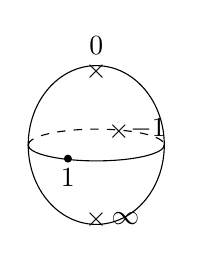
\begin{tikzpicture}[scale=.72]
\draw (0,0) ellipse (1.2 and 1.4);
\draw (-1.2,0) arc[start angle=180,end angle=360,x radius=1.2,y radius=.28];
\draw[dashed] (-1.2,0) arc[start angle=180,end angle=0,x radius=1.2,y radius=.28];
\node at (0,1.3) {$\times$}; \node[above] at (0,1.42) {$0$};
\node at (.4,.24) {$\times$};\node[right] at (.43,.28) {$-1$};
\fill (-.5,-.24) circle (2pt);\node[below] at (-.5,-.24) {$1$};
\node at (0,-1.31) {$\times$};\node[right] at (.1,-1.3) {$\infty$};
\end{tikzpicture}}

\[
z\longmapsto-\frac1{4z}(z-1)^2
\qquad \mathbb P^1(\mathbb C)\mathbin{-}\mathbb P^1(\mathbb C)
\]
(cf (23)) de sorte que l'application cherchée $X_n\longrightarrow X_0$ est
\[
\tag{92}
z\longmapsto-\frac1{4z^n}(z^n-1)^2
\]
\diagram{\begin{tikzcd}[ampersand replacement=\&]
\underbrace{X_n}_{\substack{\text{carte cycloto-}\\\text{mique type}\\\text{d'ordre }n}}
\arrow[r,"{\substack{\deleted{\unsure{g_n}}\\g_n}}"]
\&
\underbrace{X_0}_{\substack{\text{carte}\\\text{universelle}}}
\end{tikzcd}}
.\,]

Ainsi, $X_n$ devient un revêtement galoisien de $X_0$, de groupe de Galois $D_n=D_{P_0}$, ramifié comme il se doit en les seuls points $0,1,\infty$, avec en ces points la ramification $2,2,n$ respectivement, et $\Sigma_{P_0}^*=X_n^*$ devient un revêtement fini ramifié \inserted{galoisien} de $X_0\setminus\{0\}$, ramifié en les seuls points $1,\infty$, avec ramification $2,n$ en ces

\margin{86}
